% A simple template for LaTeX documents
% 
% To produce pdf run:
%   $ pdflatex paper.tex 
%

\documentclass[12pt]{article}

% Begin paragraphs with new line
\usepackage{parskip}  

% Change margin size
\usepackage[margin=1in]{geometry}   

% Graphics Example:  (PDF's make for good plots)
\usepackage{graphicx}               
% \centerline{\includegraphics{figure.pdf}}

% Allows hyperlinks
\usepackage{hyperref}

% Blocks of code
\usepackage{listings}
\lstset{basicstyle=\ttfamily, title=\lstname}
% Insert code like this. replace `plot.R` with file name.
% \lstinputlisting{plot.R}

% Monospaced fonts
%\usepackage{inconsolata}
% GNU \texttt{make} is a nice tool.

% Supports proof environment
\usepackage{amsthm}

% Allows writing \implies and align*
\usepackage{amsmath}

% Allows mathbb{R}
\usepackage{amsfonts}

% Numbers in scientific notation
% \usepackage{siunitx}

% Use tables generated by pandas
\usepackage{booktabs}

% norm and infinity norm
\newcommand{\norm}[1]{\left\lVert#1\right\rVert}
\newcommand{\inorm}[1]{\left\lVert#1\right\rVert_\infty}

% Statistics essentials
\newcommand{\iid}{\text{ iid }}
\newcommand{\Exp}{\operatorname{E}}
\newcommand{\Var}{\operatorname{Var}}
\newcommand{\Cov}{\operatorname{Cov}}


%%%%%%%%%%%%%%%%%%%%%%%%%%%%%%%%%%%%%%%%%%%%%%%%%%%%%%%%%%%%

\begin{document}

\title{Relating Traffic Events to CHP Incidents\\
ECI 256 Final Project}
\date{December 2016}
\author{Clark Fitzgerald}
\maketitle

\begin{abstract}

In this project image processing techniques were used to detect traffic
events within PeMS data for I80 West in the month of April 2016. 
These events were then related to CHP incident reports.

\end{abstract}

\section{Introduction}
%%%%%%%%%%%%%%%%%%%%%%%%%%%%%%%%%%%%%%%%%%%%%%%%%%%%%%%%%%%%

What 

A traffic event is 

\section{Review}

\cite{chung2007relation} describe traffic characteristics at three fixed bottlenecks.

\cite{chen2004systematic} describe systematic identification of bottlenecks from 5
minute loop data. We want to do a similar thing with 30 second data on a larger scale.
They use velocity measurements, which are not always reliable / available. So it might be 
better in our case to use occupancy and flow.

The say: "Five-minute data provide sufficient
resolution for this analysis because the traffic features sought are on
the order of 30 min or more." So maybe we look for finer features.

\cite{hall1991freeway} use flow and occupancy since velocity is not available.

\begin{quote}
Averages of flow and occupancy across the three lanes were
used. The two tended to vary together in the period before
congestion aud diverge during the congested period. Determining
the exact beginning and end of congestion was,
however, difficult from these numbers, so the ratio of occupancy
to flow was used. Three values of the ratio were tested
for the threshold level: 1.0, 1.1, and 1.2. A ratio of 1.0 gives
a longer duration of bottleneck flows, some of which were
very low, suggesting that demand was below capacity. A ratio
of 1.2 excludes sustained periods (10 min) of high flows (5,800
vehicles/hr or more). A ratio of 1.1 or above persisting for 3
min was selected as the criterion for the identification of the
start of a queue. 
\end{quote}

\cite{wieczorek2010techniques} applies this to Oregon data.

\cite{zhang2004some} show that Queue Discharge Flows QDF's, normal around 2K
passenger cars per lane per hour.

TODO: find papers that quantify traffic impacts of construction and various
types of accidents.

\section{Data Analysis}
%%%%%%%%%%%%%%%%%%%%%%%%%%%%%%%%%%%%%%%%%%%%%%%%%%%%%%%%%%%%

\begin{figure}
    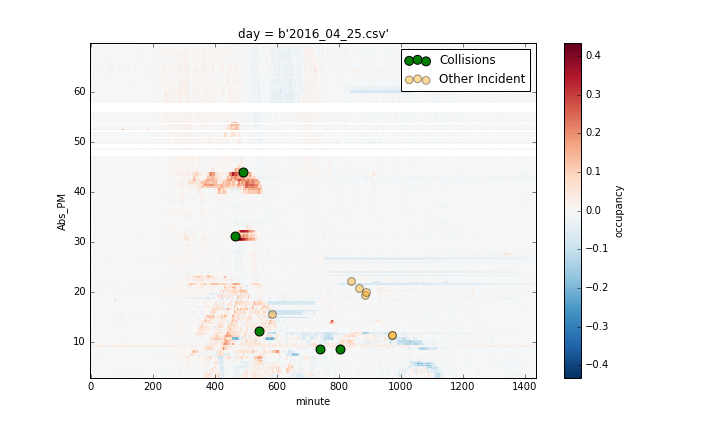
\includegraphics[scale=0.5]{../diffs.png}
    \caption{This shows the difference in occupancy from the median. Areas
    of unusually high occupancy are colored dark red.
    }
\end{figure}




\begin{figure}
    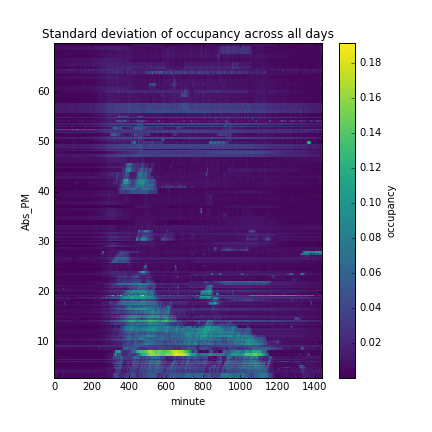
\includegraphics[scale=0.5]{../occ_sd.png}
    \caption{Occupancy varies more in areas of high traffic.}
\end{figure}


A different approach would be to treat the occupancy data as \emph{images}.
We can use opencv to do this. For each freeway we can take the following
steps:
\begin{enumerate}
    \item Use R to read the raw file and convert to an image with many missing
        values. This means expansion to a uniformly spaced grid.
    \item Interpolate missing values. 
    \item Threshold the image, so for a pixel with density $\rho >
        \rho_0$
        we define it as high density, otherwise low density. We'll
        have to experiment to see what the appropriate value of $\rho_0$ is
        but I suspect around 0.3.
    \item Once this has been done for every day we can compute an average
        thresholded image showing the areas of high density. This will show
        recurring bottlenecks. May need to threshold this also.
    \item Compare each day with the average. The difference will show the
        unusual patterns that occurred on just one day. Might have to do
        some denoising here- eliminate points that are not part of a 
        cluster.
\end{enumerate}

Once we have the denoised difference we can do the following:
\begin{enumerate}
    \item (Optional) Detect shapes that are flat on top, since this is the
        distinguishing feature of a bottleneck.
    \item Compute centroid, bounding boxes, and area which will quantify the impact
        in terms of space and time.
    \item Join these features to incident data. This likely will require some text
        analysis.
\end{enumerate}

Then we can answer questions such as:
\begin{enumerate}
    \item How many traffic events occur which have no associated incident
        data? And what sort of events were they probably?
    \item What is the impact of an event of type X on a given section of
        highway? Something along the lines of: When traffic flow is 1500
        veh per lane per hour in a two lane freeway a collision involving
        exactly two vehicles typically creates congestion lasting 10-15
        minutes which propagates back 2-3 miles. 
    \item How can we model the distribution of traffic incidents, ie.
        Poisson with some parameters.
\end{enumerate}

But how can these results be useful more broadly? More accurate
simulations. Input to real time routing. Impacts of planned construction
events. Scheduling CHP patrols and recovery services.

\section{Conclusions}
%%%%%%%%%%%%%%%%%%%%%%%%%%%%%%%%%%%%%%%%%%%%%%%%%%%%%%%%%%%%


My favorite broad idea: Empirically quantify the impact of various flow levels on congestion.
I suspect that for a given type of accident total delay experienced by
travelers increases superlinearly as a function of (flow / capacity).
Assuming we're looking at uncongested regions. If this holds then it can be
used as an argument that we need to try to keep (flow / capacity) under
some level. This could mean taking measures such as toll roads or tax
credits for employers who find ways to keep employees off roads during peak
commute hours. My favorite- an argument to make cars more expensive (like
tolls and mileage tax) and use money to improve public transportation.

Why is this interesting? Interdisciplinary since we combine data munging,
computer vision, and statistics. Provides motivation for developing
automatic R / C++ bindings that I'll be working on. Has legitimate possible
impacts. Most computer vision stuff in traffic works on real cameras.
Haven't seen any papers that use it for this.

\bibliography{citations} 

\bibliographystyle{apalike}

\end{document}
